The term ``fake lepton'' denotes here generically non-prompt leptons produced in heavy flavor meson decays, 
converted photons, light hadrons faking the electron shower, in-flight decays of kaons or pions to muons, etc.  
Common properties shared by these objects are a bad response to the electron/muon identification cuts, 
non-zero impact parameters, and the reconstructed leptons are often not well isolated. 
These properties can be used to discriminate the fake leptons against the prompt and isolated leptons we are interested in (and which we call ``real leptons''). 

We rely on two different and complementary methods to estimate the fake leptons yields in the signal regions, 
either purely data-driven or relying on the MC simulations, 
which are described respectively in Sections~\ref{sec:bkg_matrix_method} and~\ref{sec:bkg_mctemplate_method}; 
we also cross-check the fake background estimate for the special case of the SR3b signal region with a third method described in section~\ref{sec:bkg_abcd_method}. 
First two methods have already been employed successfully in the Run-1 analysis~\cite{noteSS3L}. 
The rest of this section provides some details about the dominant sources of fake leptons close to the signal regions according to the simulations predictions. 


%%%%%%%%%%%%%%%%%%%%%%%%%%%%%
\subsubsection{Fake lepton sources close to the signal regions} 
\label{sec:truthComposition_SR}

We studied in the MC simulations the sources of fake leptons close to the signal regions, which we briefly summarize here. 
This information is important notably for the setup of the related background estimate (the matrix method) and the assignment of systematic uncertainties. 
It is also genuinely interesting as it may help further rejecting fake leptons by focusing on the relevant source and devising appropriate discriminants. 

Ideally we would study directly the composition of the signal regions; 
however, the limited MC statistics does not really allow to do so with a high level of confidence on the results. 
Therefore, to have more reliable conclusions, we performed these studies in a set of regions with relaxed selection criteria compared to the signal regions (i.e. no \meff\ cut, looser cuts on ($b$-) jet multiplicity and \met, etc.). 
Such criteria are detailed in Table~\ref{tab:TruthComposition_SR}. 
However, the conclusions obtained in this section can be extrapolated to the signal regions, 
notably since the source of fake leptons due to $t\bar t$ processes dominates over other sources both in the relaxed and in the ``nominal'' signal regions. 

The sources of fake leptons are identified through the classification performed by the \texttt{MCTruthClassifier} tool, 
following the approach defined in section~\ref{sec:truth_matching}. 
In this present section, only \ttbar\ and $V$+jets Monte Carlo samples (as presented in Section~\ref{sec:BGSamples}) are analysed, 
since we expected the other potential sources (QCD processes such as $pp\to b\bar b$, diboson\ldots) to be very minor in the signal regions. 
To increase the available statistics, we did not apply the requirements on the charges of the leptons here. 

\begin{table}[h!]
\caption{The relaxed signal regions used to study the origin of fake leptons in simulation.}
\hspace{0.5cm}
\label{tab:TruthComposition_SR}
\centering
%\resizebox{0.8\textwidth}{!}{
\begin{tabular}{|c|c|c|c|}
\hline
\hline
Signal region  &      $N_{lept}$             & $N_{b-jets}^{20}$               & Other variables \\
\hline
\hline
SR0b &  $\ge$2  &    $==$0        &     $N_{jets}^{25} \ge$ 3, \met\ ~$>$~70 \GeV \\
\hline
SR1b     &  $\ge$2  &    $\ge$1        &     $N_{jets}^{25} \ge$ 3, \met\ ~$>$~70 \GeV \\
\hline
SR2b     &   $\ge$2  &   $\ge$2        &   -    \\
\hline
\end{tabular}%}
\end{table}
 

\par{\bf Fake electron sources\\}
The fake electrons are classified in a few general categories depending on the origin of the electron 
(conversion from prompt photons, light hadron fakes including $\pi^0\to\gamma\gamma$, non-prompt taus, bottom and charm meson semileptonic decays). 
The relative abundances of these sources are shown in Fig~\ref{Fig:truthComposition_EL_by_source_vs_pt} for different $p_T$ cuts on the electrons, 
in the relaxed signal regions defined in Table~\ref{tab:TruthComposition_SR}. 
They are presented for both baseline and signal electrons definitions~--~the former being useful to understand the events input to the matrix method in the signal regions. 
For completeness, the number of events in each category and the associated statistical uncertainties 
are shown in Appendix~\ref{App:FakeLep} (Fig~\ref{Fig:truthComposition_EL_by_source_vs_pt_MORE}). 
The dependency on other kinematic variables like \met, \meff, etc. is shown in the same appendix. 

Generally a strong dependency is observed on the fake electron \pt. 
At the baseline level, in the relaxed SR0b and SR1b regions 
the dominant sources of fake electrons arise from both light hadron fakes and bottom hadrons decays; 
however, at the signal level the dominant source is the bottom hadrons decays, beside at high \pt\ ($>$30~\GeV) where the light flavor sources are higher than 30\%. In a selection with $\ge 2$ $b$-jets, most of the fakes arise from light hadrons decays.
%, apart in the low \pt region (as low as 10~\GeV) at signal level where bottom decays contribute equally.

Fig~\ref{Fig:truthComposition_EL_pT_spectrum} presents the $p_T$ spectrum of the fake electrons in the relaxed signal regions, 
distinguishing the $t\bar t$ and $V+$ jets processes. 
In all signal regions the background will be dominated by fake electrons from \ttbar processes. 
The first \pt bin ($p_T<20$ GeV) is depleted since due to the $p_T$ requirements in the lepton selection, 
only events with three leptons may fill this bin, which are less frequent in \ttbar. 

\begin{figure}[p]
\centering
\subfigure[Baseline electrons, ``relaxed'' SR0b] 
{\includegraphics[width=0.49\textwidth]{Truth_Composition/Baseline/Vj_1EL_pT_Var_DEF4.pdf}}
\subfigure[Signal electrons, ``relaxed'' SR0b]{
\includegraphics[width=0.49\textwidth]{Truth_Composition/Signal/Vj_1EL_pT_Var_DEF4.pdf}
}
\subfigure[Baseline electrons, ``relaxed'' SR1b]
{\includegraphics[width=0.49\textwidth]{Truth_Composition/Baseline/Vj_1EL_pT_Var_DEF5.pdf}}
\subfigure[Signal electrons, ``relaxed'' SR1b]{
\includegraphics[width=0.49\textwidth]{Truth_Composition/Signal/Vj_1EL_pT_Var_DEF5.pdf}
}
\subfigure[Baseline electrons, ``relaxed'' SR2b]
{\includegraphics[width=0.49\textwidth]{Truth_Composition/Baseline/Vj_1EL_pT_Var_DEF6.pdf}}
\subfigure[Signal electrons, ``relaxed'' SR2b]{
\includegraphics[width=0.49\textwidth]{Truth_Composition/Signal/Vj_1EL_pT_Var_DEF6.pdf}
}
\caption
{Sources of fake electron as a function of the electron $p_T$, as predicted by MC simulations (combined $t\bar t$ and $V+$ jets) 
in the relaxed signal regions defined in Table~\ref{tab:TruthComposition_SR}. The results are shown for baseline (left) or signal electrons (right).} 
\label{Fig:truthComposition_EL_by_source_vs_pt}
\end{figure}
%%
\begin{figure}[p]
\centering
\subfigure[Baseline electrons, ``relaxed'' SR0b]
{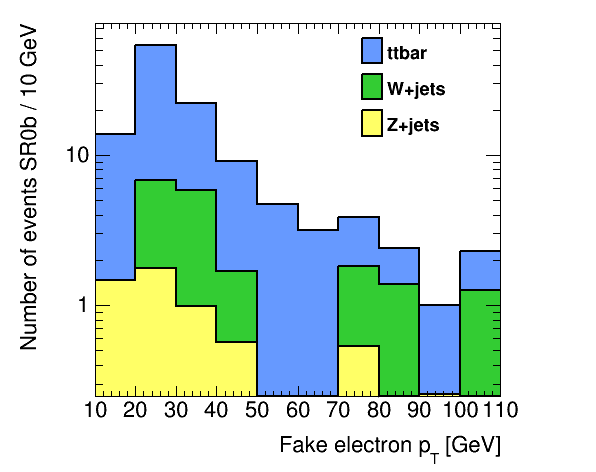
\includegraphics[width=0.49\textwidth]{Truth_Composition/BaseEL_SR0bPt}}
\subfigure[Signal electrons, ``relaxed'' SR0b]{
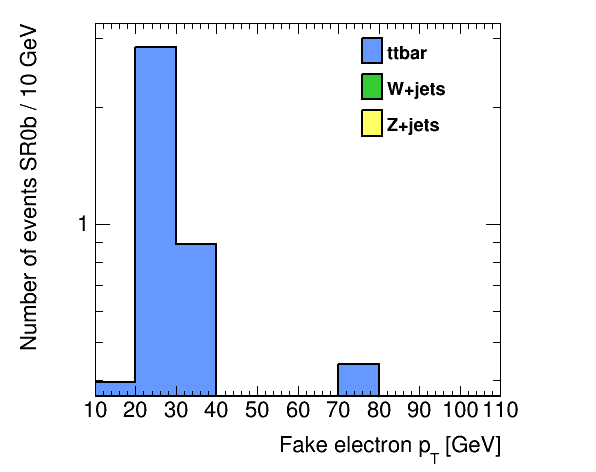
\includegraphics[width=0.49\textwidth]{Truth_Composition/SigEL_SR0bPt}
}
\subfigure[Baseline electrons, ``relaxed'' SR1b]
{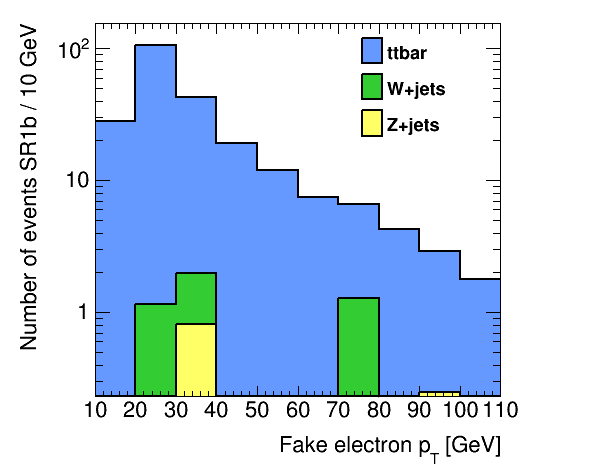
\includegraphics[width=0.49\textwidth]{Truth_Composition/BaseEL_SR1bPt}}
\subfigure[Signal electrons, ``relaxed'' SR1b]{
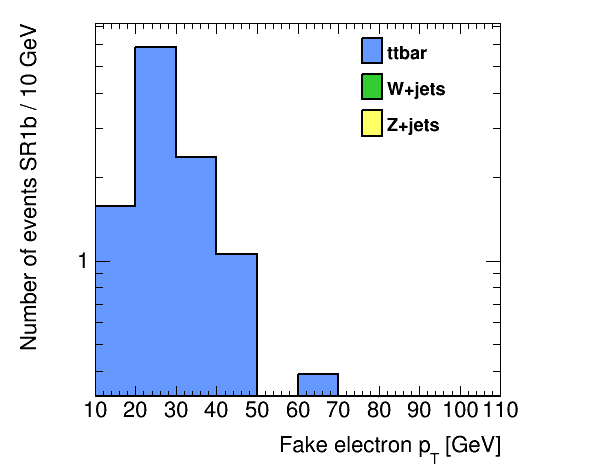
\includegraphics[width=0.49\textwidth]{Truth_Composition/SigEL_SR1bPt}
}
\subfigure[Baseline electrons, ``relaxed'' SR2b]
{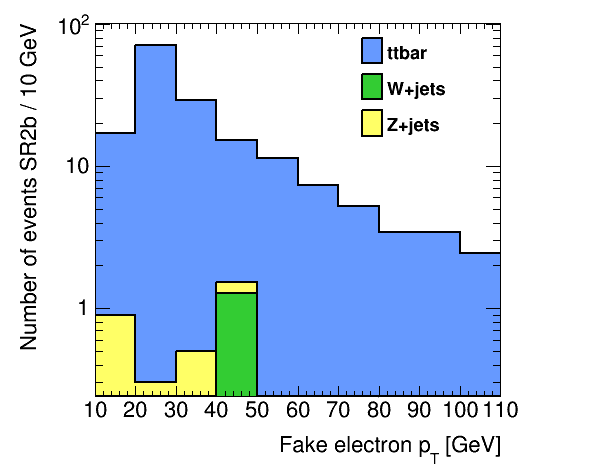
\includegraphics[width=0.49\textwidth]{Truth_Composition/BaseEL_SR2bPt}}
\subfigure[Signal electrons, ``relaxed'' SR2b]{ 
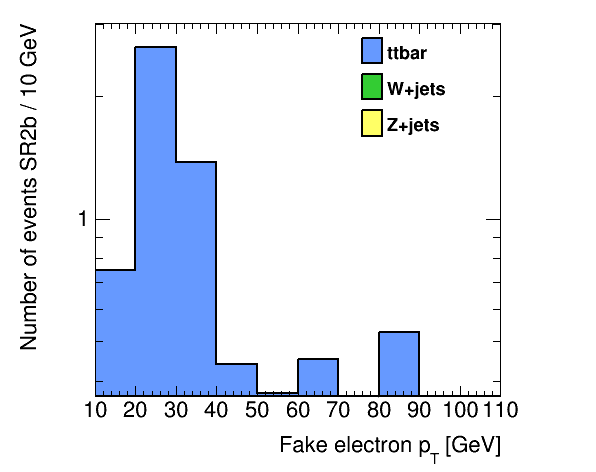
\includegraphics[width=0.49\textwidth]{Truth_Composition/SigEL_SR2bPt}
}
\caption
{Transverse momentum distribution of the fake electrons as predicted by MC simulations in the relaxed signal regions defined in Table~\ref{tab:TruthComposition_SR}. Electrons originating from $t\bar t$ or $V+$ jets events are distinguished. }
\label{Fig:truthComposition_EL_pT_spectrum}
\end{figure}


\par{\bf Fake muon sources\\}
We classified fake muons into four categories, according to the decision of the \texttt{MCTruthClassifier} tool, and depending on the heavy flavor content of the hadron at the origin of the muon (light, tau, bottom and charm). We show the relative abundances of these sources in Fig~\ref{Fig:truthComposition_MU_by_source_vs_pt} for different $p_T$ cuts on the muons, in the relaxed signal regions defined in Table~\ref{tab:TruthComposition_SR}. They are presented for both baseline and signal muons definitions. The number of events in each category and the associated statistical uncertainties are shown in Appendix~\ref{App:FakeLep} (Fig~\ref{Fig:truthComposition_MU_by_source_vs_pt_MORE}). The dependency of other kinematic variables like \met, \meff, etc. is shown in the same appendix.

One can see that the dominant source are always non-prompt muons arising from charmed or bottom hadron decays, in all \pt regions. In general, the non-prompt muons come mainly from $b$-sources (the fraction of such events is around 70$\%$ or more), 
except in the SR2b selection: this is interpreted as the fact that in $t\bar t$ events, tagging the 2 $b$-jets (as is required in this region) strongly reduces the rate of non-prompt muons originating from these, as the small impact parameter required for that muon to satisfy signal cuts contradicts the $b$-jet tagging which relies on the presence of displaced tracks and a secondary vertex. Fig~\ref{Fig:truthComposition_MU_pT_spectrum} presents the $p_T$ spectrum of these fake muons in the relaxed signal regions, distinguishing the $t\bar t$ and $V+$ jets processes. For all selections, the background will be dominated by low $p_T$ fake muons originating from $t\bar t$. 

\begin{figure}[p]
\centering
\subfigure[Baseline muons, ``relaxed'' SR0b]
{\includegraphics[width=0.49\textwidth]{Truth_Composition/Baseline/Vj_1MU_pT_Var_DEF4.pdf}}
\subfigure[Signal muons, ``relaxed'' SR0b]{
\includegraphics[width=0.49\textwidth]{Truth_Composition/Signal/Vj_1MU_pT_Var_DEF4.pdf}
}
\subfigure[Baseline muons, ``relaxed'' SR1b]
{\includegraphics[width=0.49\textwidth]{Truth_Composition/Baseline/Vj_1MU_pT_Var_DEF5.pdf}}
\subfigure[Signal muons, ``relaxed'' SR1b]{
\includegraphics[width=0.49\textwidth]{Truth_Composition/Signal/Vj_1MU_pT_Var_DEF5.pdf}
}
\subfigure[Baseline muons, ``relaxed'' SR2b]
{\includegraphics[width=0.49\textwidth]{Truth_Composition/Baseline/Vj_1MU_pT_Var_DEF6.pdf}}
\subfigure[Signal muons, ``relaxed'' SR2b]{
\includegraphics[width=0.49\textwidth]{Truth_Composition/Signal/Vj_1MU_pT_Var_DEF6.pdf}
}
\caption
{Sources of fake muons as a function of the muon $p_T$, as predicted by MC simulations (combined $t\bar t$ and $V+$ jets) 
in the relaxed signal regions defined in Table~\ref{tab:TruthComposition_SR}. The results are shown for baseline (left) or signal muons (right).}
\label{Fig:truthComposition_MU_by_source_vs_pt}
\end{figure} 
%%
\begin{figure}[p]
\centering
\subfigure[Baseline muons, ``relaxed'' SR0b]
{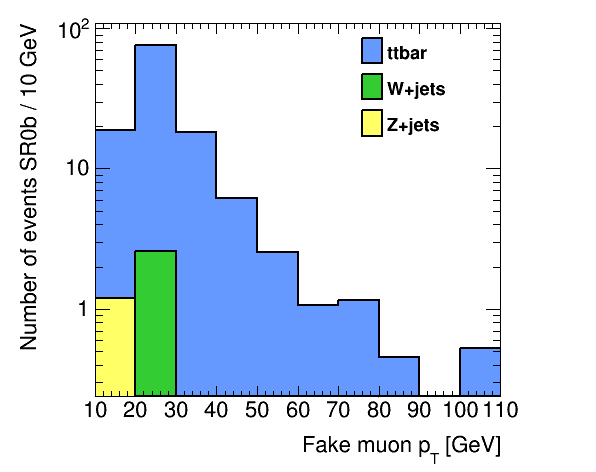
\includegraphics[width=0.49\textwidth]{Truth_Composition/BaseMU_SR0bPt}}
\subfigure[Signal muons, ``relaxed'' SR0b]{
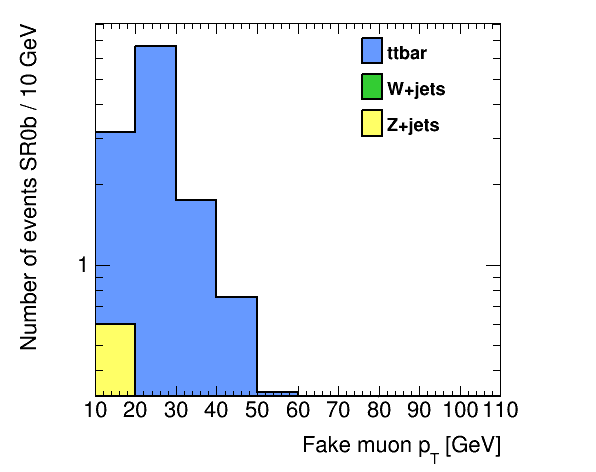
\includegraphics[width=0.49\textwidth]{Truth_Composition/SigMU_SR0bPt} 
}
\subfigure[Baseline muons, ``relaxed'' SR1b]
{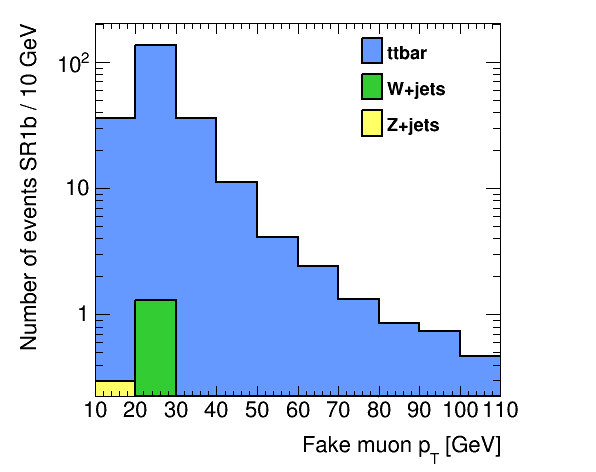
\includegraphics[width=0.49\textwidth]{Truth_Composition/BaseMU_SR1bPt}}
\subfigure[Signal muons, ``relaxed'' SR1b]{
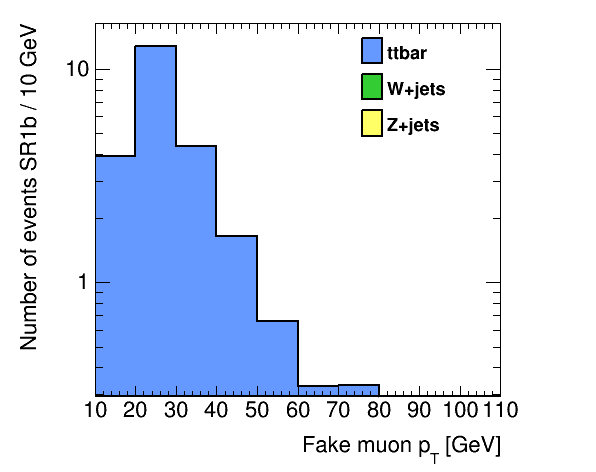
\includegraphics[width=0.49\textwidth]{Truth_Composition/SigMU_SR1bPt}
}
\subfigure[Baseline muons, ``relaxed'' SR2b]
{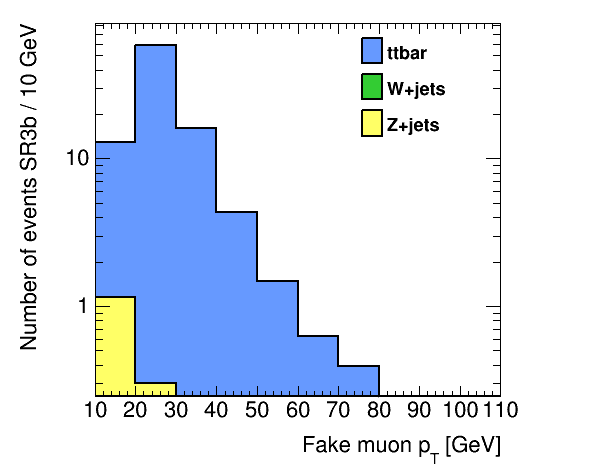
\includegraphics[width=0.49\textwidth]{Truth_Composition/BaseMU_SR2bPt}}
\subfigure[Signal muons, ``relaxed'' SR2b]{
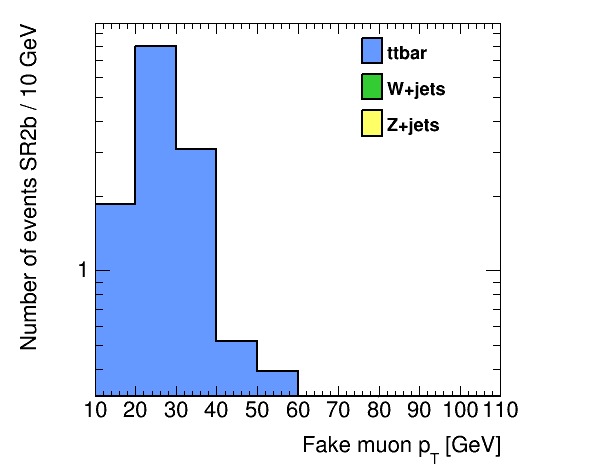
\includegraphics[width=0.49\textwidth]{Truth_Composition/SigMU_SR2bPt}
}
\caption
{Transverse momentum distribution of the fake muons as predicted by MC simulations in the relaxed signal regions defined in Table~\ref{tab:TruthComposition_SR}. Muons originating from $t\bar t$ or $V+$ jets events are distinguished. }
\label{Fig:truthComposition_MU_pT_spectrum}
\end{figure} 

%%%%

